\section{The W/Z-Tagging algorithm}
\label{sec: W/Z tagging}

The products of hadronic decays of $\wboson$ bosons can
fall within a single jet if these particles are boosted relative to
their mass.  The $\wboson$ tagging algorithm is developed to
identify these boosted $\wboson$ jets, based on the removal of the softest
components of the jets (jet pruning)~\cite{catop_cms,topwtag_pas}.

The jet pruning algorithm uses the CA $R=0.8$ jets
as inputs. In the process, soft and
wide-angle particles (relative to the parent in the clustering) are
ignored.  The same parameters are chosen for the jet pruning algorithm
as in the original theoretical papers~\cite{jetpruning1,jetpruning2}.

The following selection is then applied on the pruned jets
to identify jets from hadronic W/Z decays:

\begin{itemize}

\item {\bf Pruned jet mass}  $\mbox{\boldmath$m_{\text{jet}}$}$
  - Require the total pruned jet mass to satisfy $70 \GeVcc < m_\text{jet} <  100 \GeVcc $.

\item {\bf N-subjettiness} 
  - Require the 2nd-subjettiness/1st-subjettiness $<$ 0.5 for the ungroomed CA8 jets. 
\end{itemize}

A detailed performance study of this W-tagger has been made public in Ref.~\cite{JME-13-006}.

\subsection{N-subjettiness}
\label{sec:N-subjettiness}

N-subjettiness~\cite{Thaler:2010tr,Thaler:2011gf,Stewart:2010tn} exploits the fact that the pattern of the hadronic decay of a heavy object is reflected through the presence of distinctive energy lobes corresponding to the decay products, as opposed to QCD jets which present a more uniformly spread energy configuration( not aligned along the subjet axis). The inclusive jet shape N-subjettiness is defined, in its generalized version as derived in ~\cite{Thaler:2010tr}, as 
%
\begin{equation}
\tau_N = \frac{1}{d_{0}} \sum_{k} p_{T,k}\,min( (\Delta R_{1,k})^{\beta}, (\Delta R_{2,k})^{\beta}...(\Delta R_{N,k})^{\beta})
\end{equation}
%
where the index $k$ runs over the jet constituents and the distances
$\Delta R_{n,k}$ are calculated with respect to the axis of the $n^{\mathrm{th}}$
subjet. The normalization factor $d_{0}$ is calculated as $d_{0}=
\sum_{k} p_{T,k}R^{\beta}_{0}$, setting $R_{0}$ to the jet radius of
the original jet. In the analysis, the N-subjettiness is calculated
from the ungroomed jets with the parameter $\beta=1$. In particular,
the variable able to best discriminate between $\PW/\cPZ$ jets and QCD jets
is the ratio of 2-subjettiness over 1-subjettiness,
$\tau_{21}=\tau_{2} / \tau_{1}$, which turns out to be smaller for signal than for background as demonstrated in Fig.~\ref{fig:N-sub-mass}.

\begin{figure}[htb]
\centering
\begin{tabular}{cc}
     \resizebox{0.5\linewidth}{!}{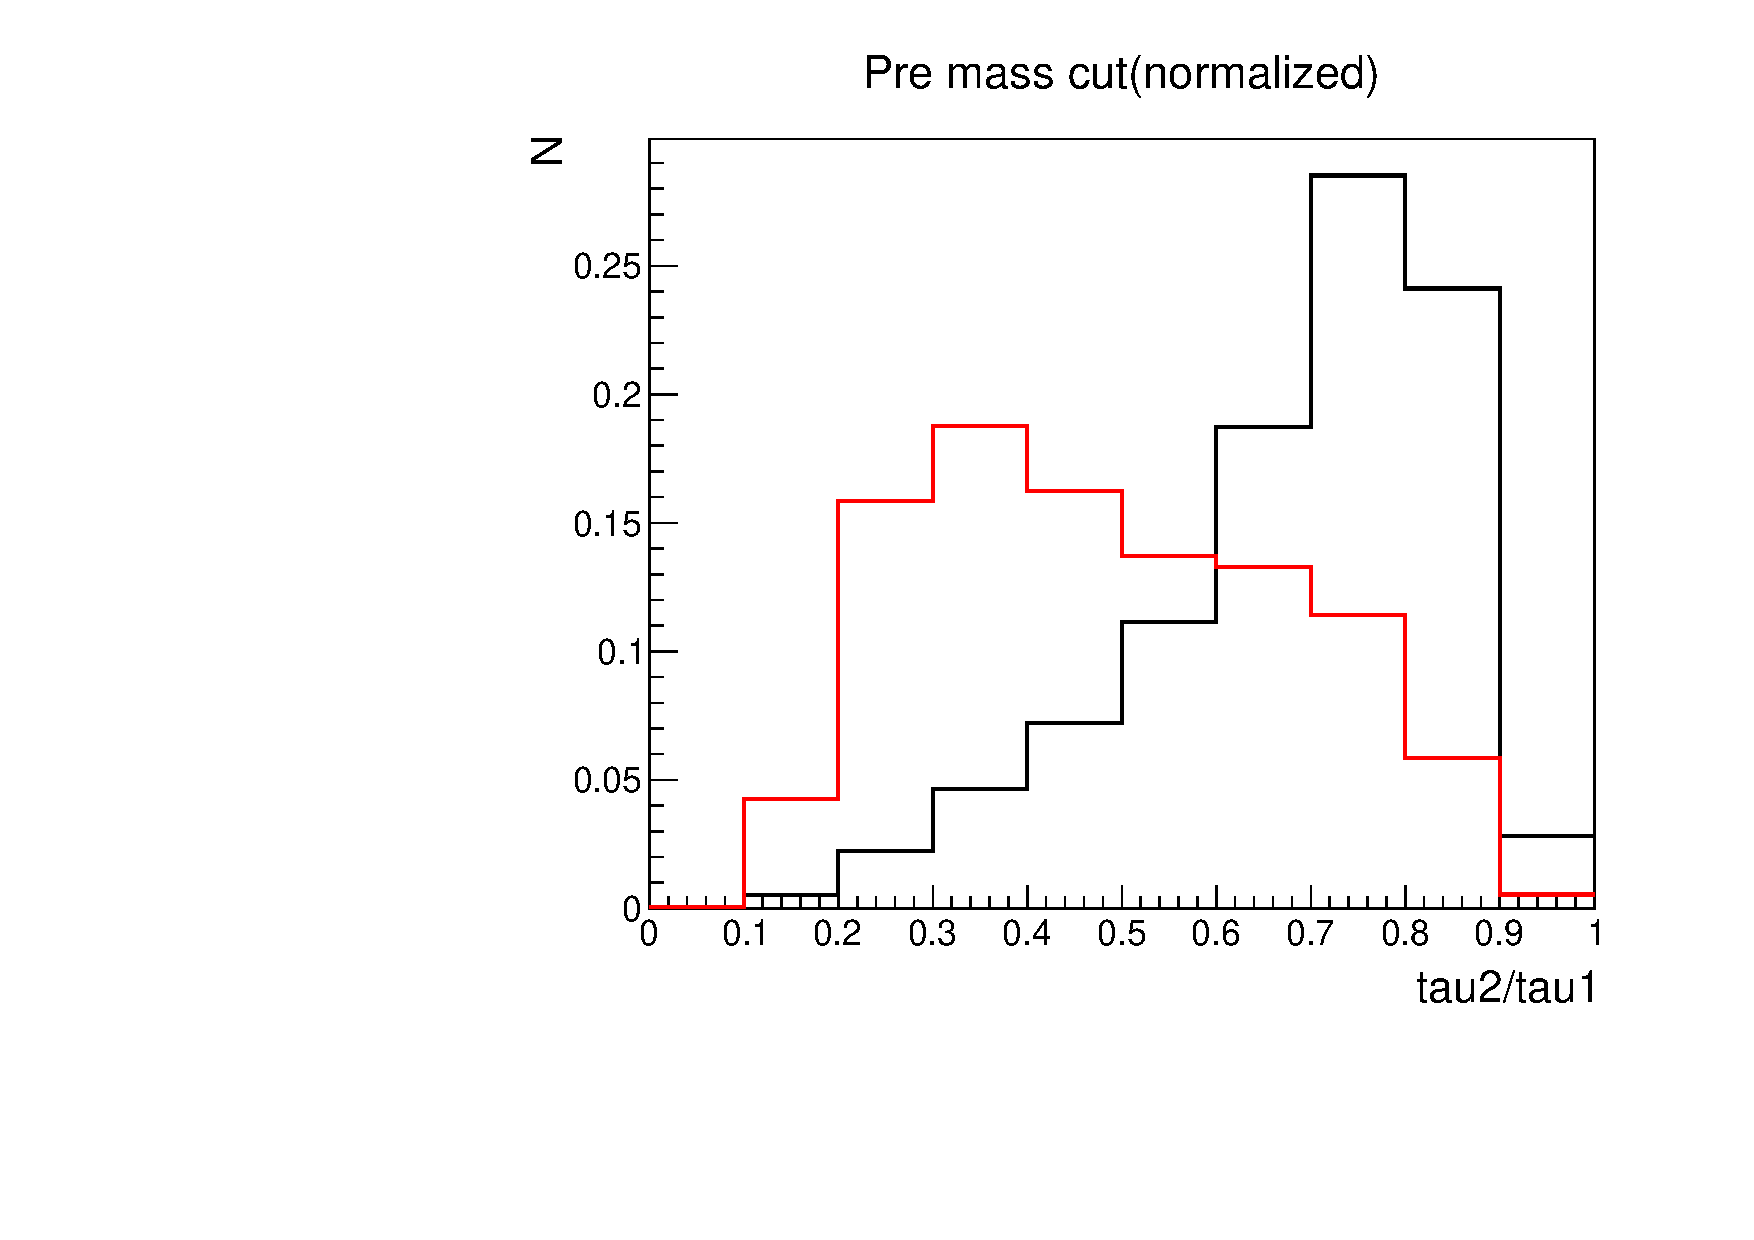
\includegraphics{figs/N-subjettiness/Signal_MC_Pre.pdf}} &
     \resizebox{0.5\linewidth}{!}{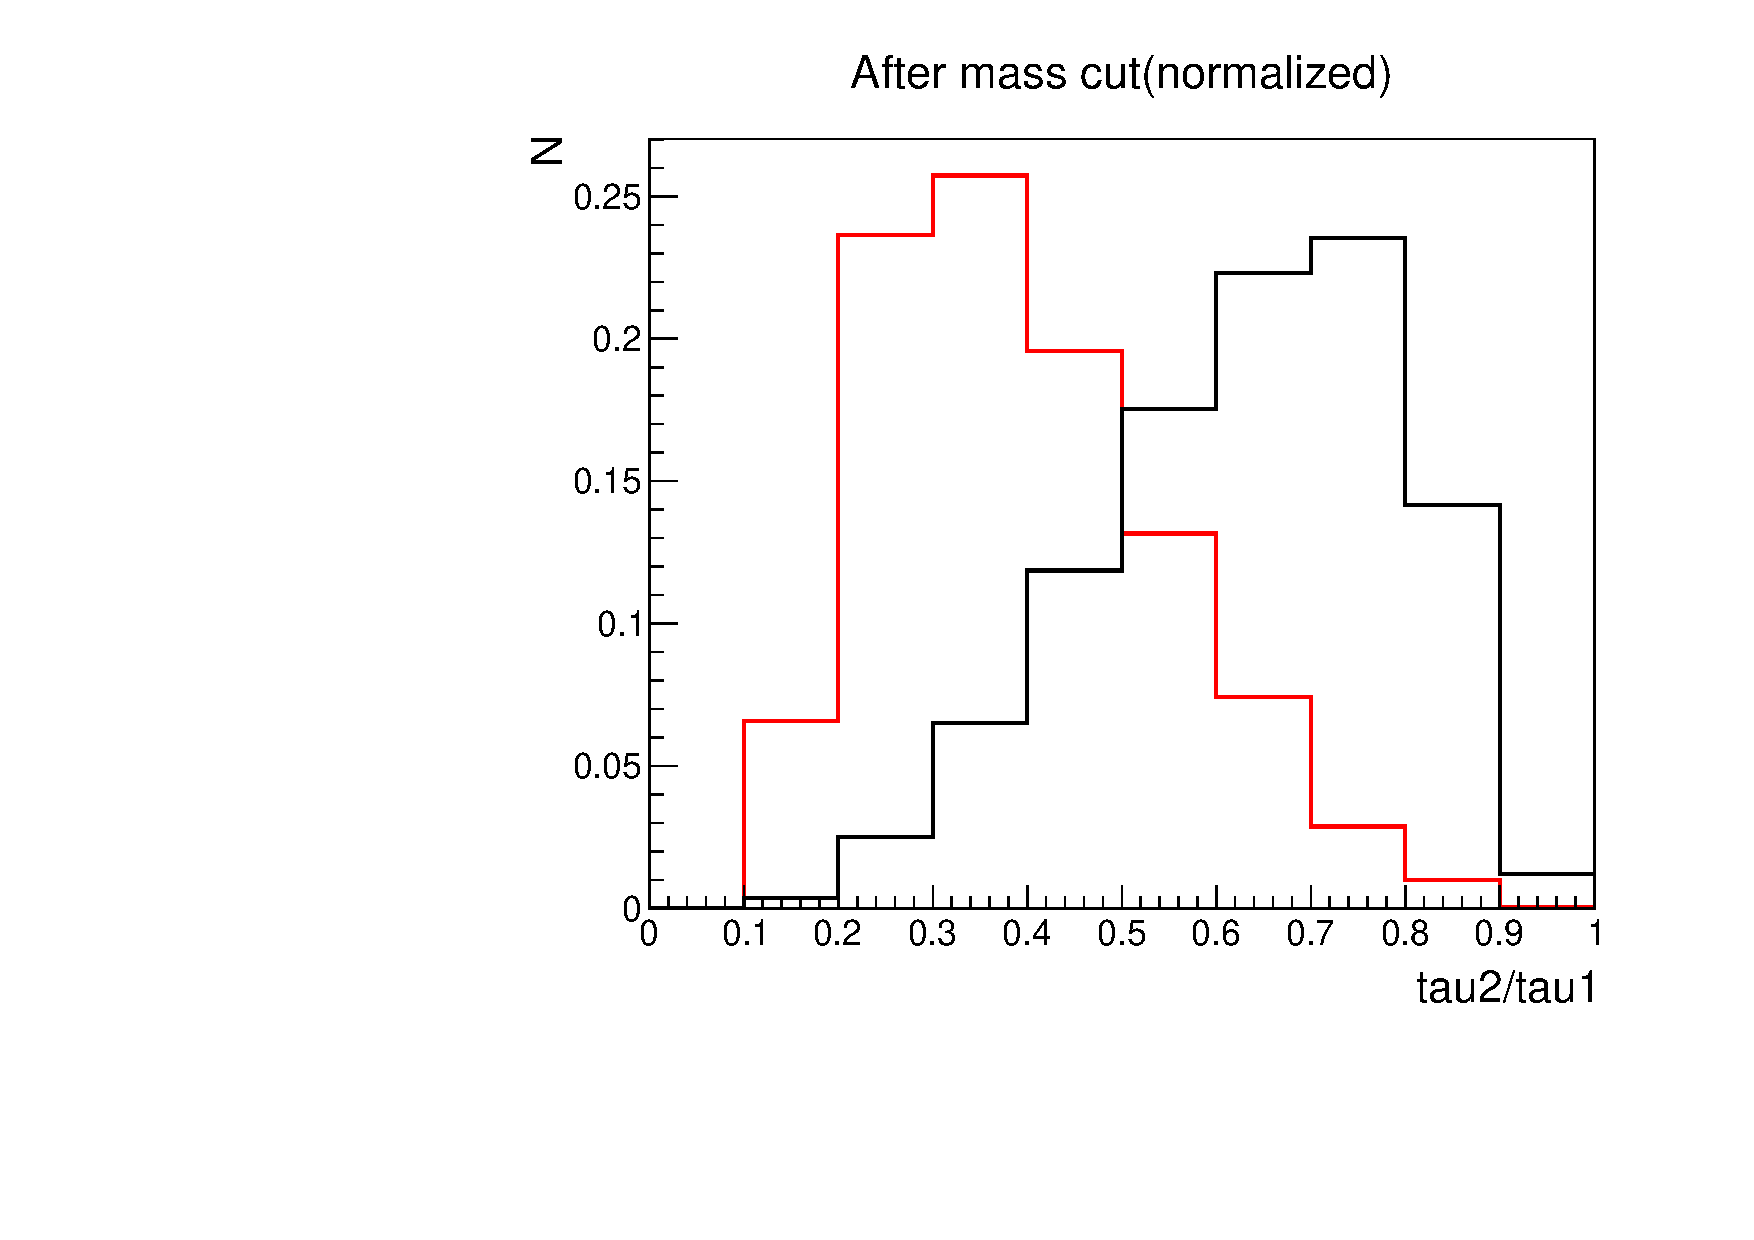
\includegraphics{figs/N-subjettiness/Signal_MC.pdf}} \\
\end{tabular}
\caption[N-subjettiness]{Comparison for $\tau_{2}/\tau_{1}$ distribution between signal (red) and background (black) before the jet mass cut (left) and after the jet mass cut applied (right). The signal MC used here is Herwig WW 1.5 TeV, and background is Herwig QCD.}
\label{fig:N-sub-mass}
\end{figure}

%\textbf{PLAN} in Fig~\ref{N-sub} and Fig~\ref{N-sub-mass}, I'm gonna add prettier plots for different signals(pythia and herwig, 1.0Tev to 3.0TeV resonance).  

%The leading two ungroomed CA8 jets to the leading two pruned CA8 jets are matched requireing $\Delta R < 0.5 $, which fails in less than 0.1\% of the events.

We select ``high purity'' $\PW/\cPZ$ jets by
requiring $\tau_{21} \leq 0.5$, while $ 0.5 <
\tau_{21} < 0.75$ defines the ``low purity'' $\PW/\cPZ$ jets.
%
The division of events with one $\PW/\cPZ$-tag follows the same delineation.
%
The events with two $\PW/\cPZ$-tagged jets are always required 
to have one high purity $\PW/\cPZ$ tag, and are similarly divided
into a ``high'' and ``low purity'' categories depending on whether
the other $\PW/\cPZ$-tagged jet is high or low purity.
%
The high purity category has been optimized to reach on average the
best sensitivity for all models considered in this search.  The low
purity category adds sensitivity in particular at high dijet masses
where the $\PW/\cPZ$-tagging efficiency drops along with the
background rate.

\subsection{Optimization study for the W-tagger}
\label{sec:optimal}
%\textbf{PLAN} This part we're gonna talk about what we did for the optimization search of tau2/tau1 cut. 

The cut values for the pruned jet mass and n-subjettiness were optimized based on the best expected limit.
The final cut values are a compromise between best expected limits for WW and ZZ resonances in the range between 1 and 2 TeV, because we target both of them with the same analysis.

Figure~\ref{fig:optimization0} shows the optimization of the n-subjettiness ($\tau_{21}$) or massdrop ($\mu$) cut value.
The massdrop variable was used in the 2011 version of this analysis and has been replaced by the n-subjettiness.
A n-subjettiness cut gives a ~30\% better limit than the massdrop cut.
$\tau_{21}<0.5$ is the best cut value for equal performance in both WW and ZZ resonances.
The expected limit changes by $<$5\% changing the $\tau_{21}$ cut value by $\pm$0.05.
The related analyses EXO-12-021 and EXO-12-022 also found $\tau_{21}<0.5$ as the optimial cut value for W- and Z-tagging.

\begin{figure}[htb]
\centering
\begin{tabular}{cc}
     \resizebox{0.5\linewidth}{!}{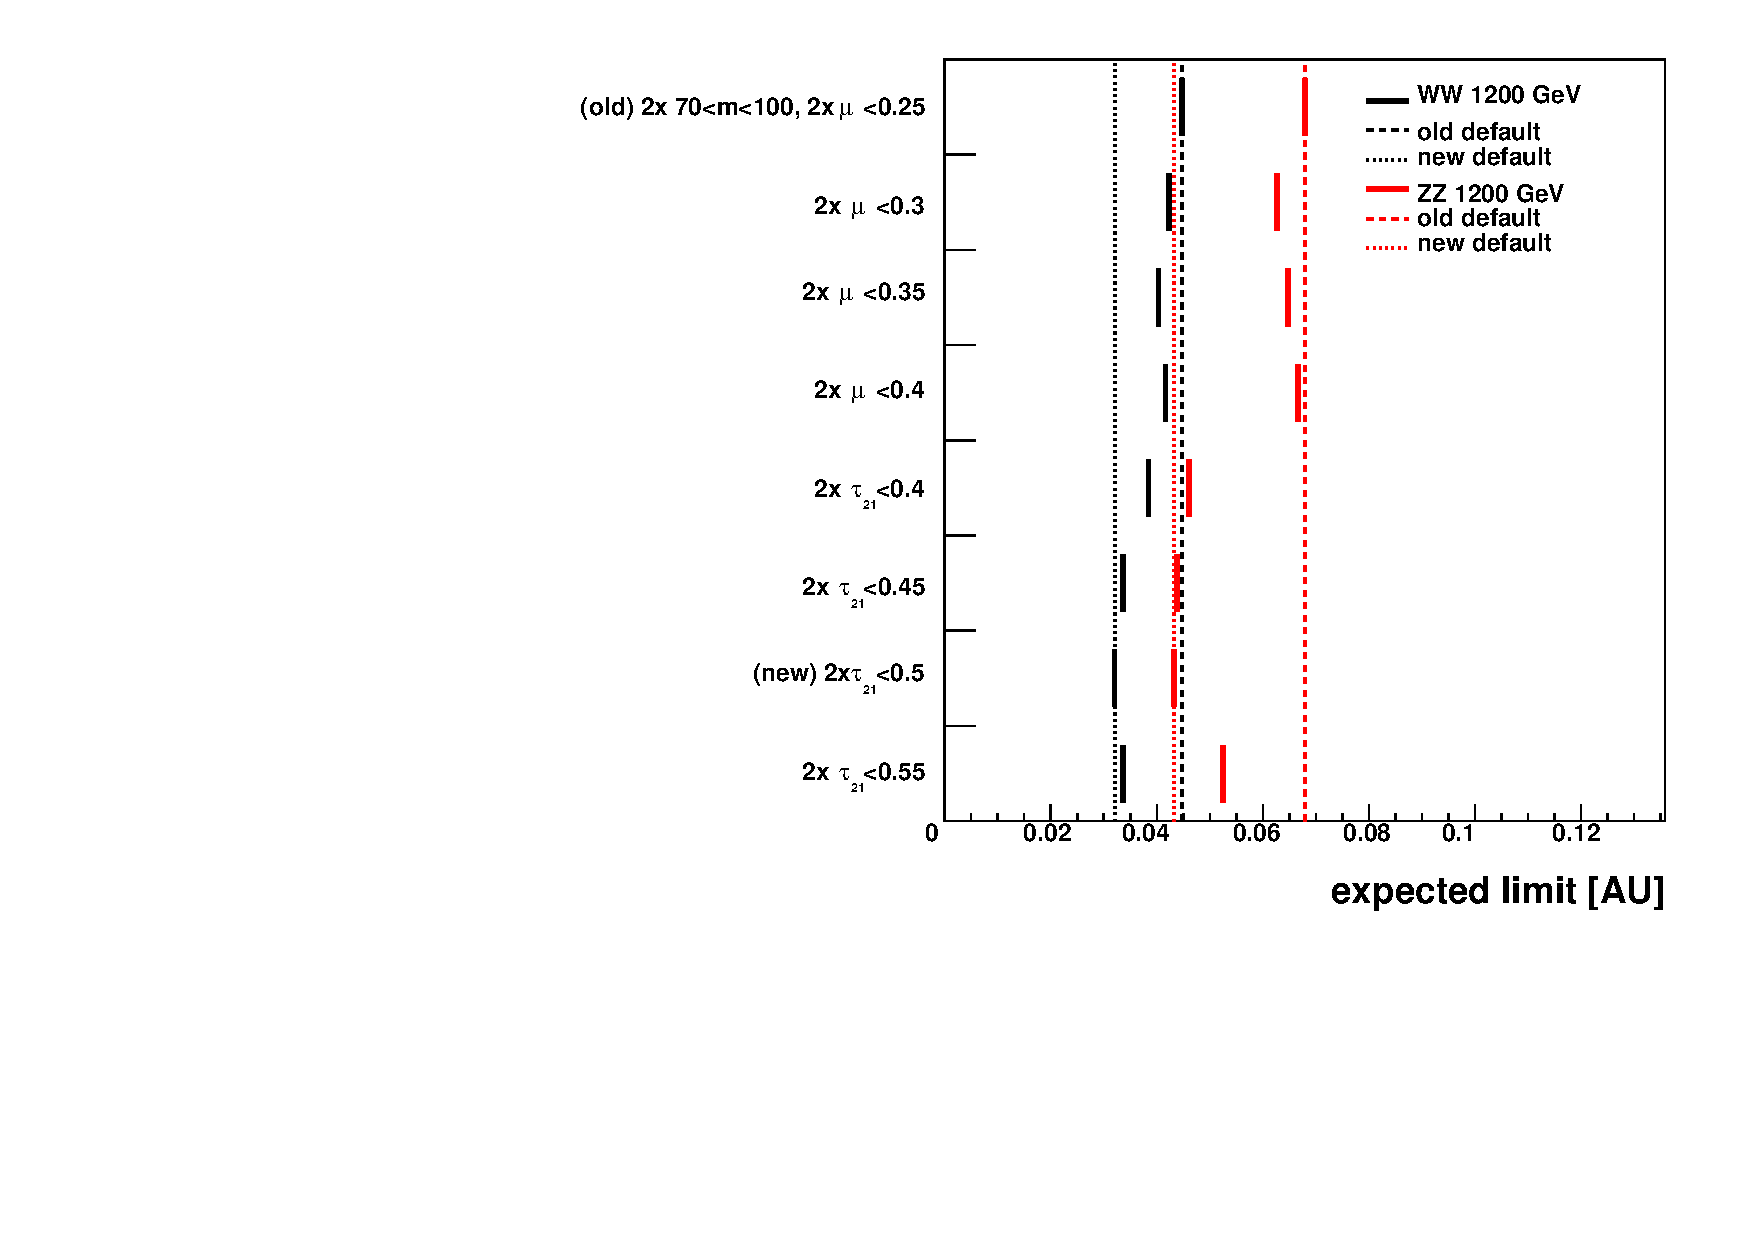
\includegraphics{figs/N-subjettiness/optimization1200_0.pdf}} &
%     \resizebox{0.5\linewidth}{!}{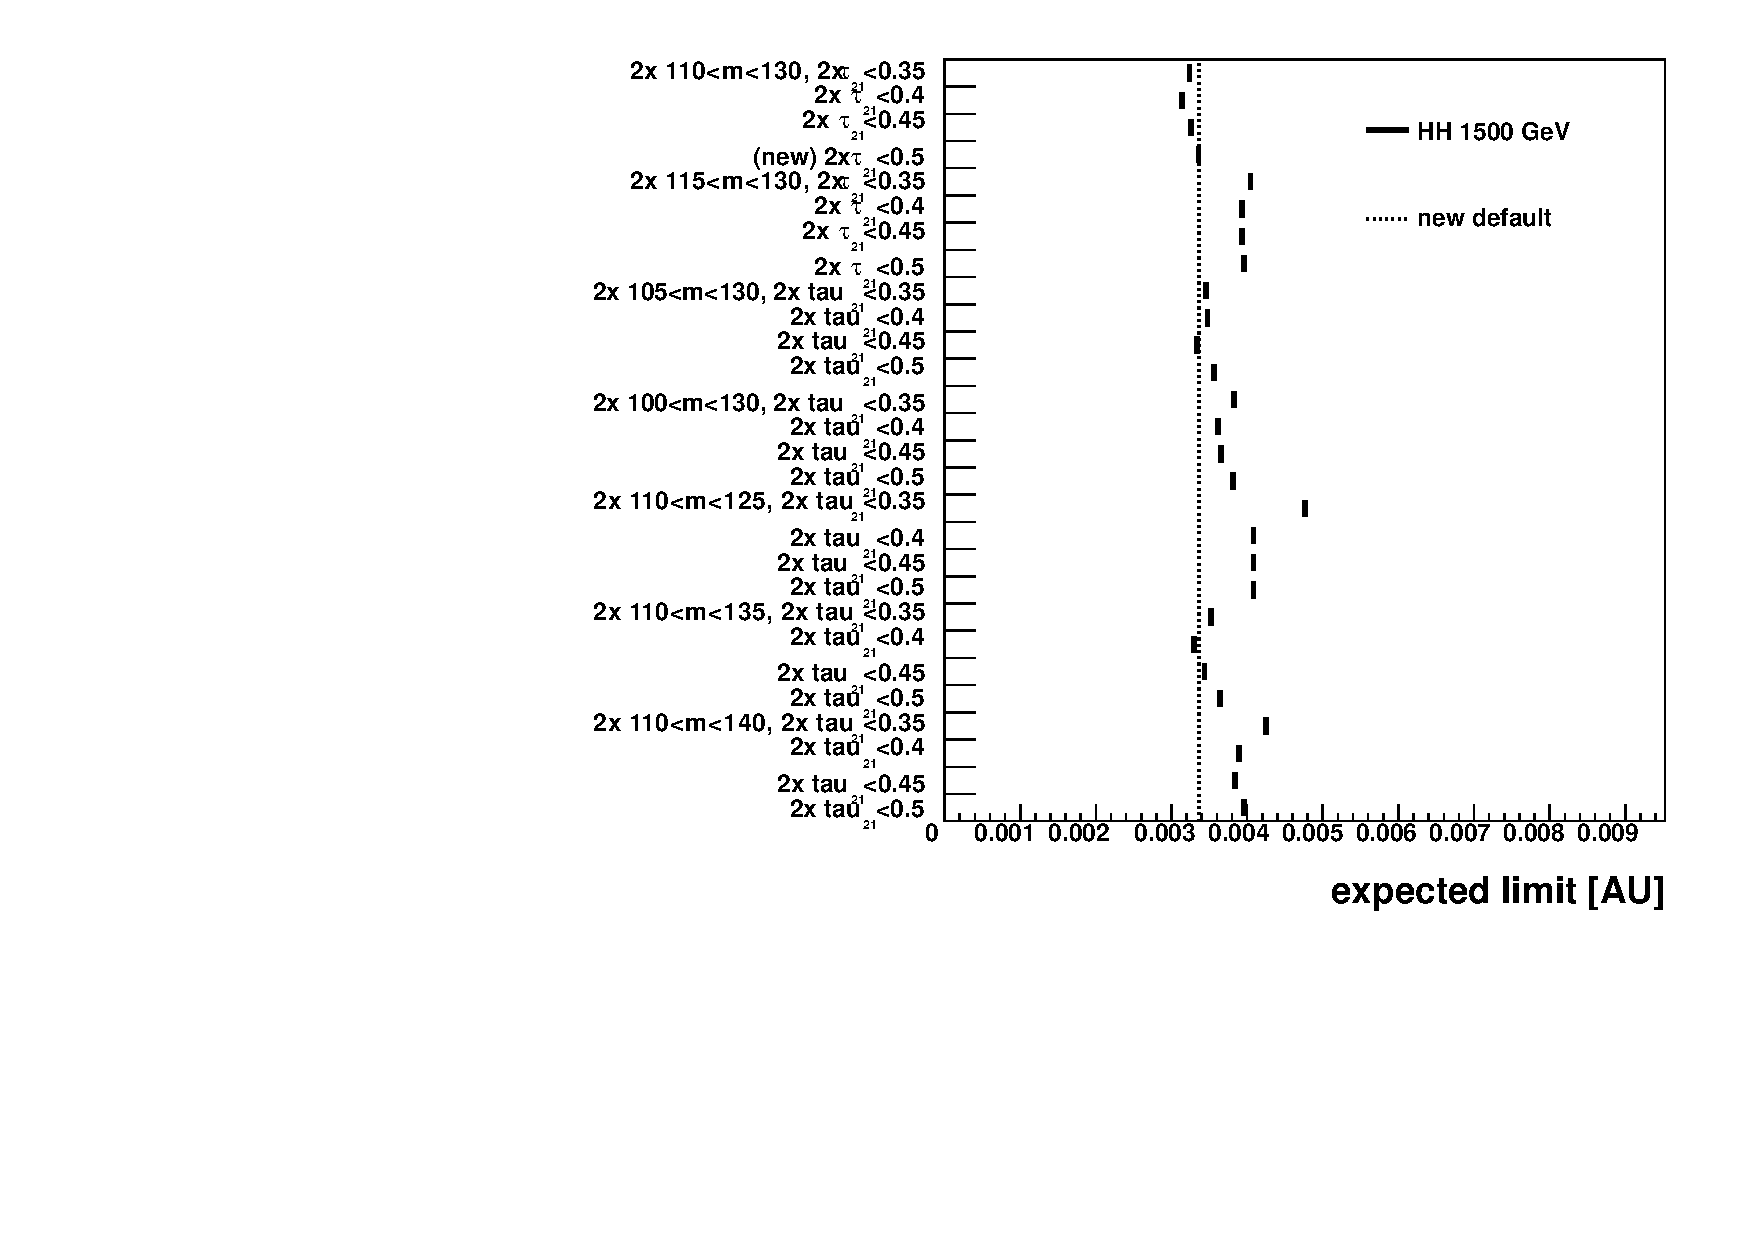
\includegraphics{figs/N-subjettiness/optimization1500_0.pdf}} &
     \resizebox{0.5\linewidth}{!}{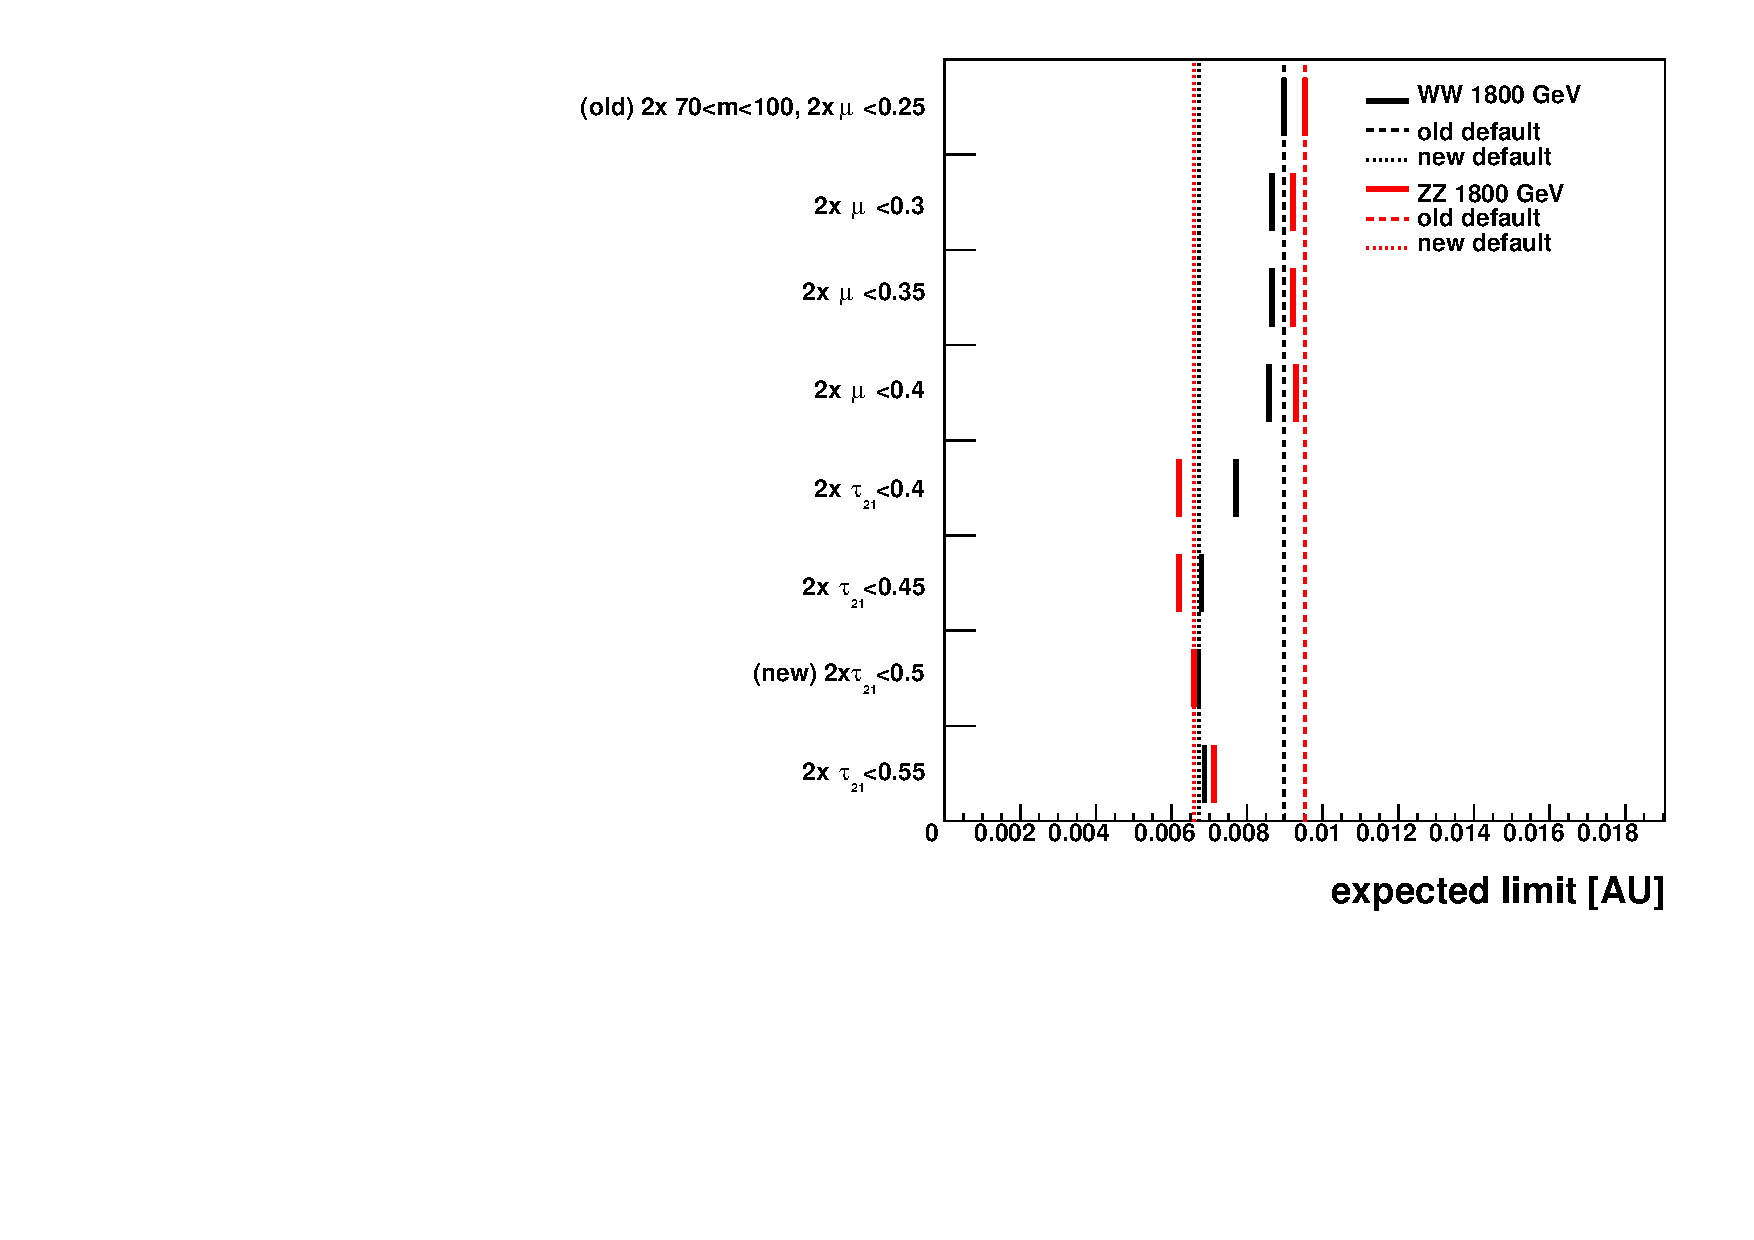
\includegraphics{figs/N-subjettiness/optimization1800_0.pdf}} \\
\end{tabular}
\caption[N-subjettiness]{Optimizataion of the n-subjettiness ($\tau_{21}$) or massdrop ($\mu$) cut value for the best expected limit.}
\label{fig:optimization0}
\end{figure}

Figure~\ref{fig:optimization1} shows the optimization of the pruned jet mass window cut.
Neither wideing nor narrowing the pruned jet mass window on either side can improve the expected limit for WW and ZZ at the same time.
The jet mass window of $70 \GeVcc < m_\text{jet} <  100 \GeVcc $ provides best performance for WW and ZZ at the same time.

\begin{figure}[htb]
\centering
\begin{tabular}{cc}
     \resizebox{0.5\linewidth}{!}{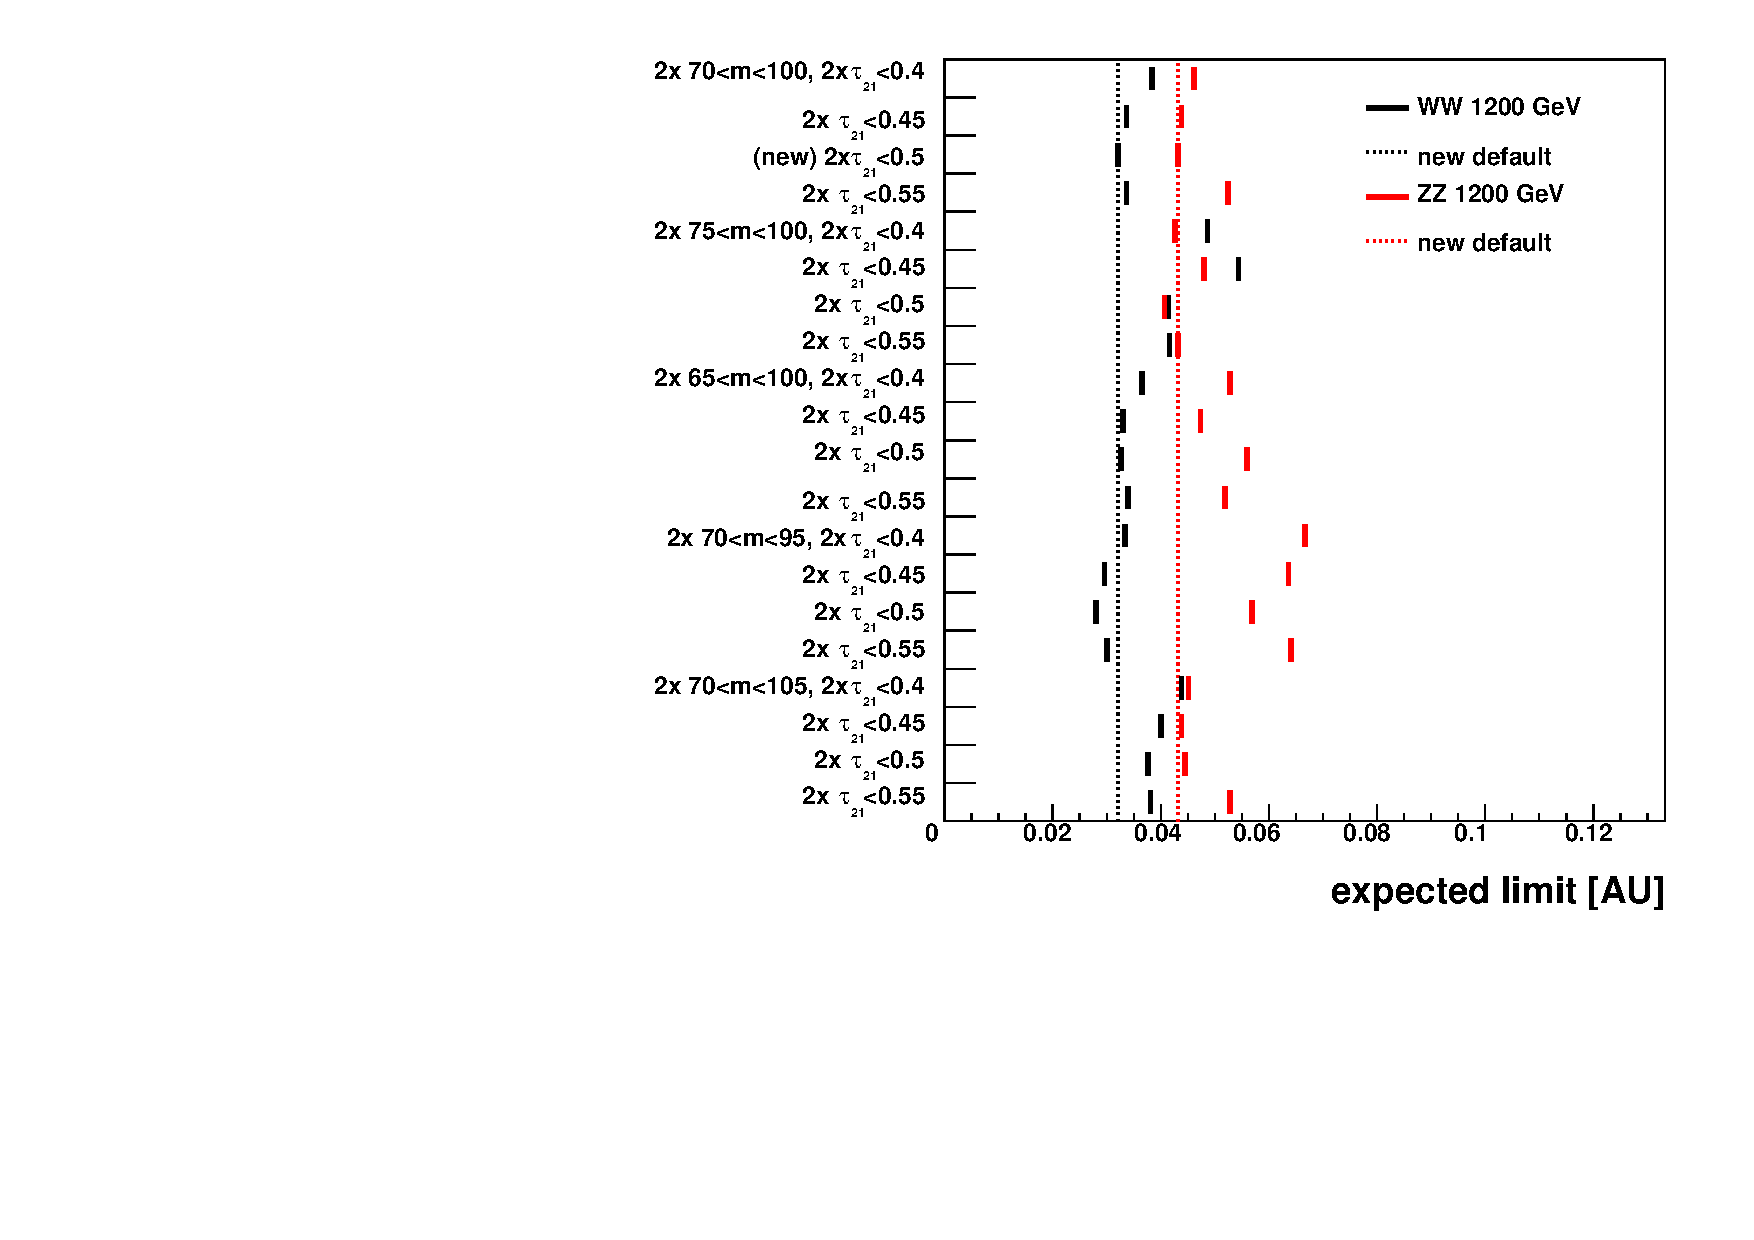
\includegraphics{figs/N-subjettiness/optimization1200_1.pdf}} &
%     \resizebox{0.5\linewidth}{!}{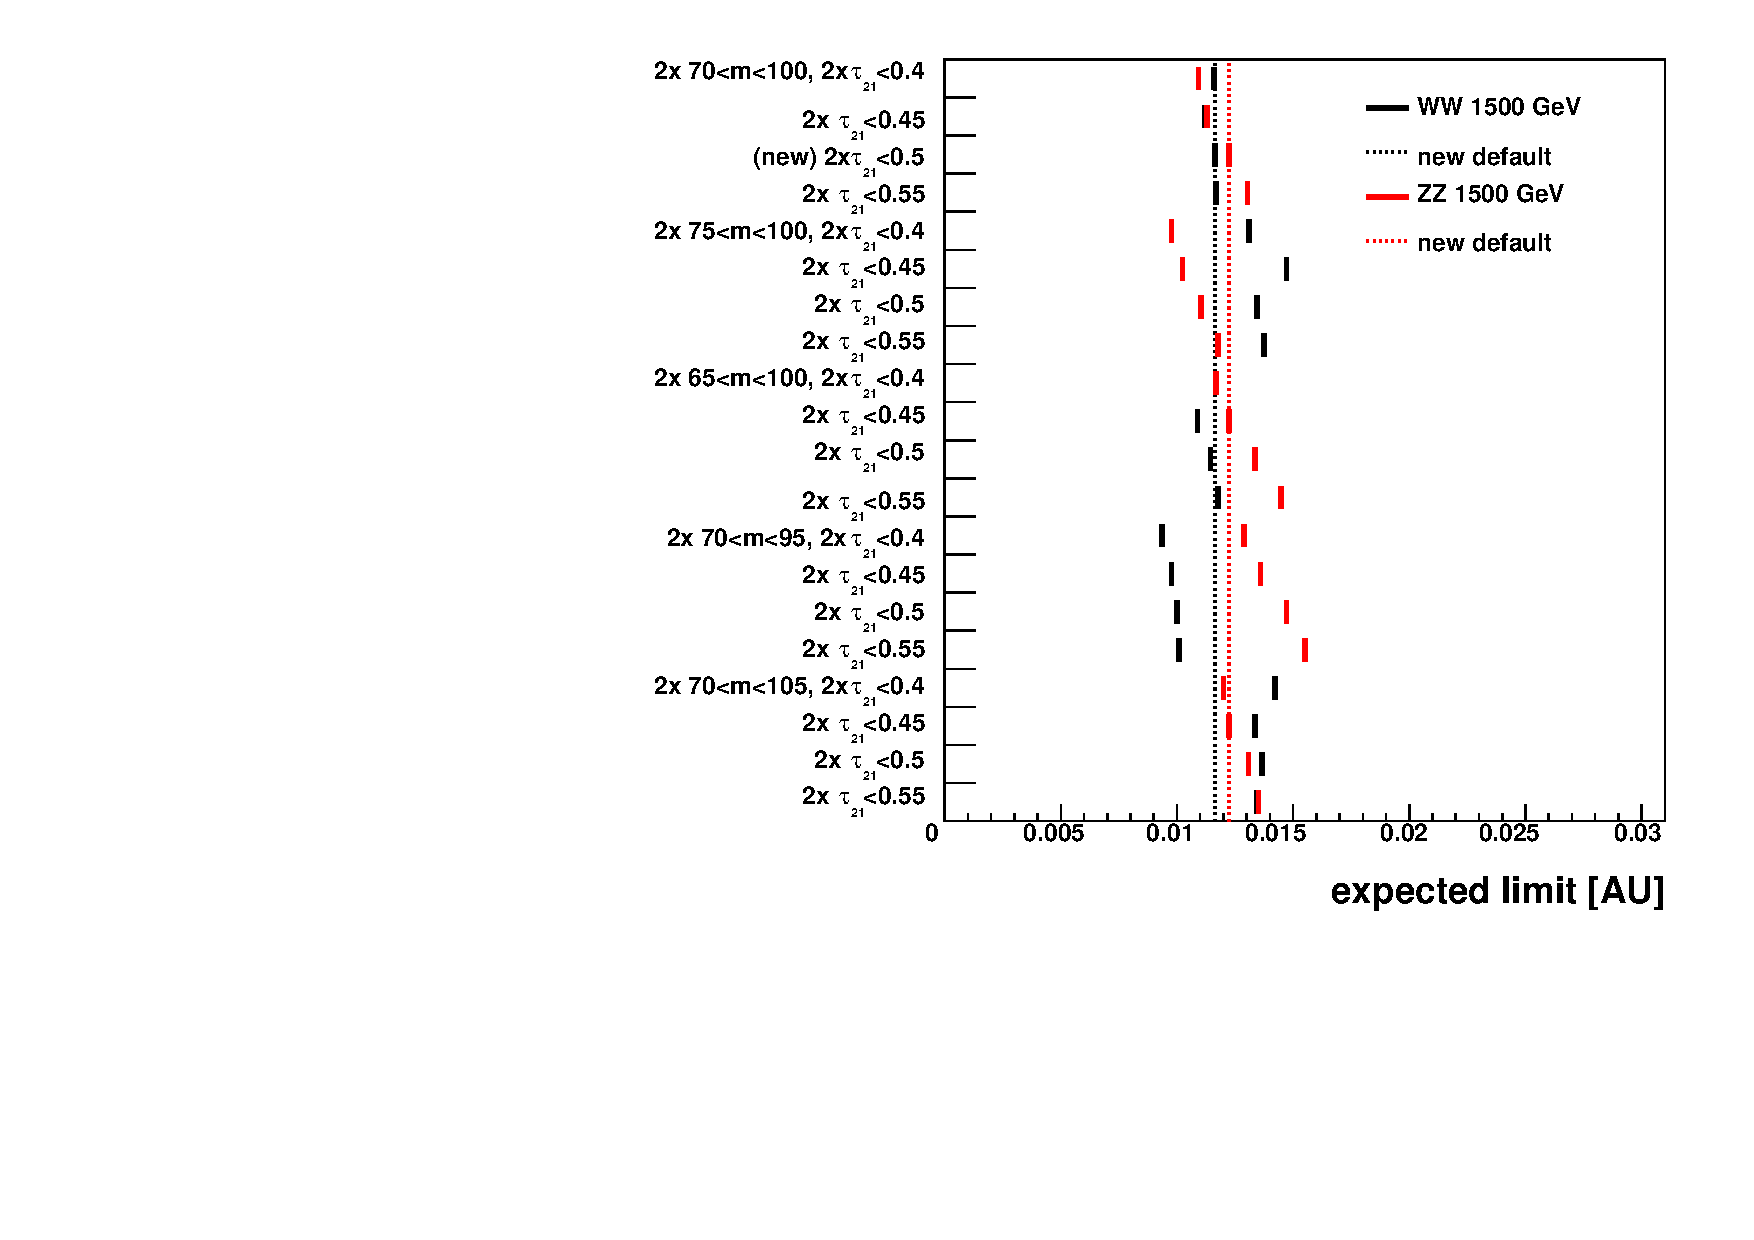
\includegraphics{figs/N-subjettiness/optimization1500_1.pdf}} &
     \resizebox{0.5\linewidth}{!}{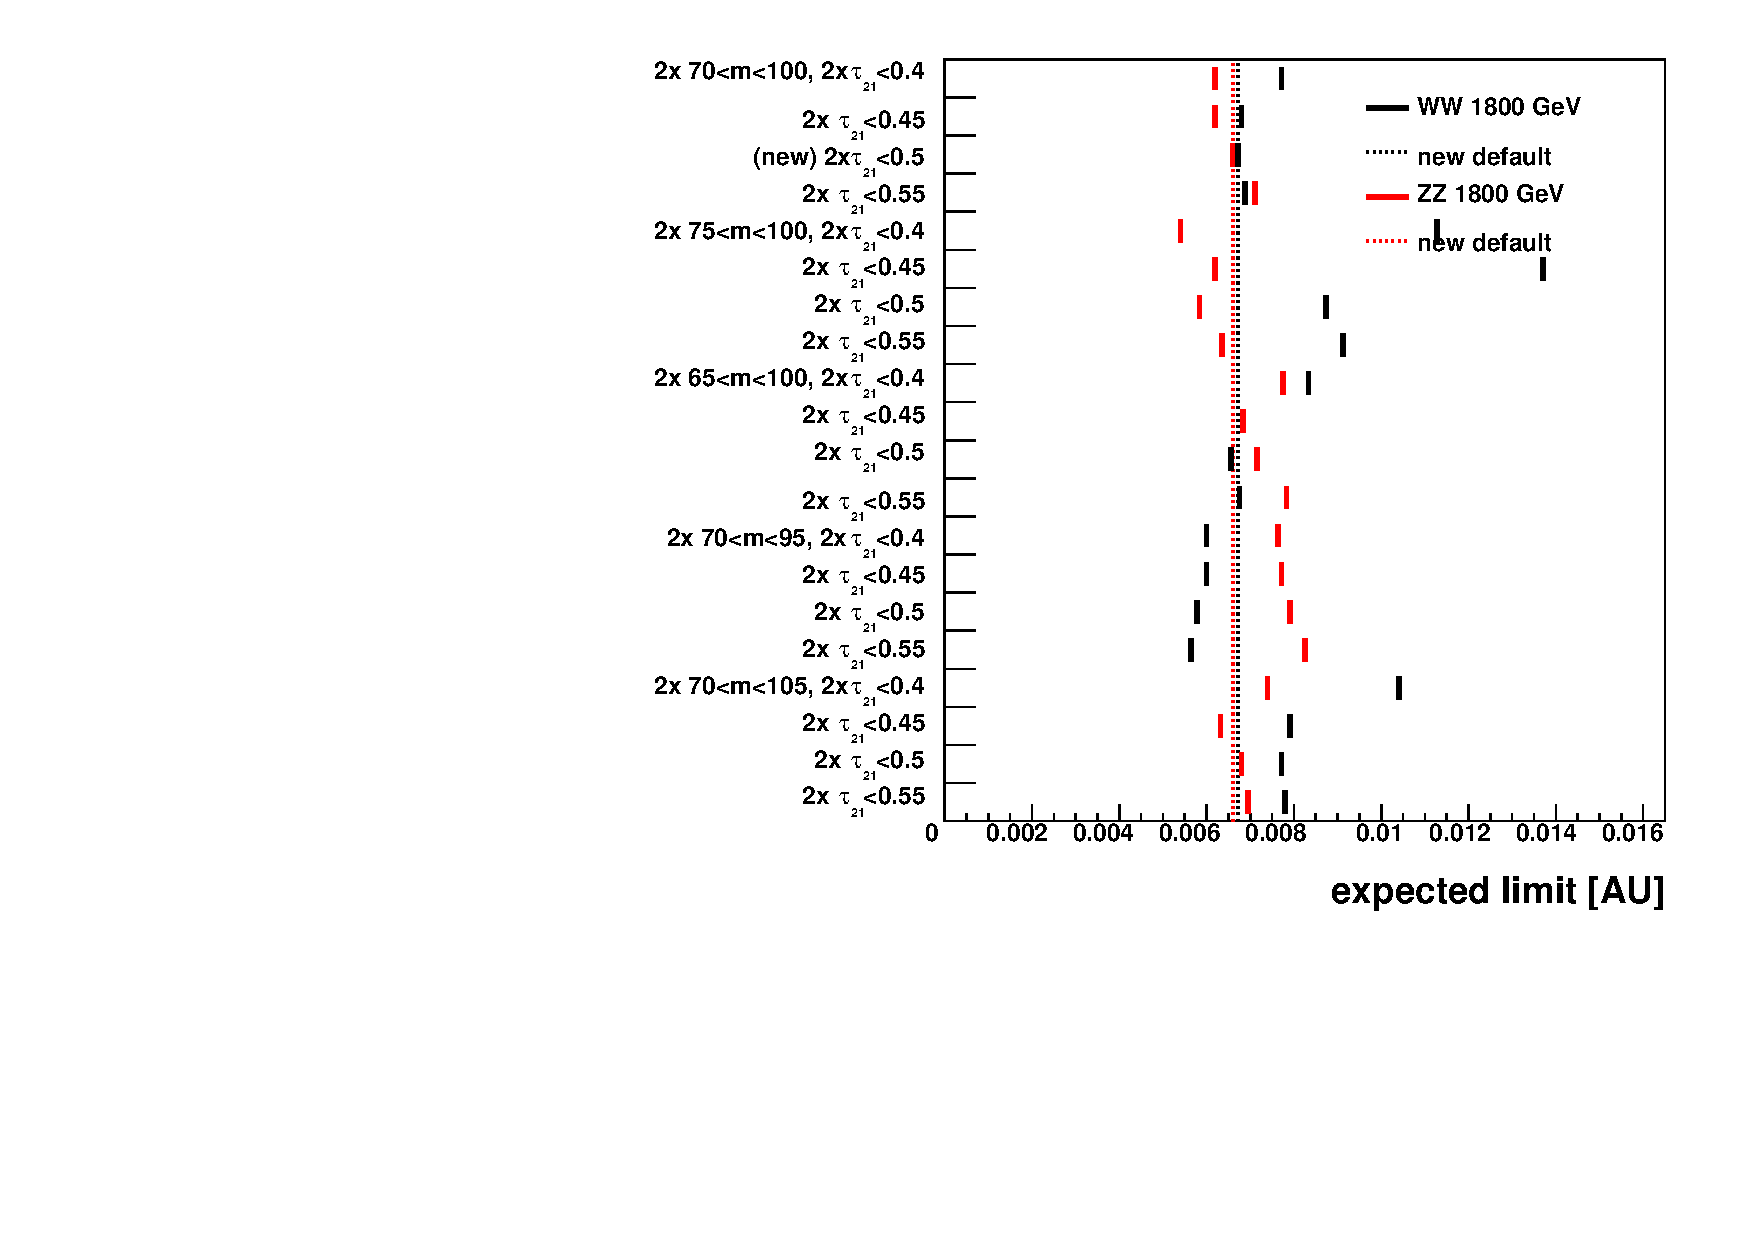
\includegraphics{figs/N-subjettiness/optimization1800_1.pdf}} \\
\end{tabular}
\caption[N-subjettiness]{Optimizataion of the pruned jet mass window cut for the best expected limit.}
\label{fig:optimization1}
\end{figure}

Figure~\ref{fig:optimization2} shows the dependency of the expected limit on the jet algorithm used for the resonance mass reconstruction.
It is found that AK5, AK7 and CA8 show almost the same performance.
This analysis switched since 2011 from AK5 to CA8 for consistency with EXO-12-021 and EXO-12-022.

\begin{figure}[htb]
\centering
\begin{tabular}{cc}
%     \resizebox{0.5\linewidth}{!}{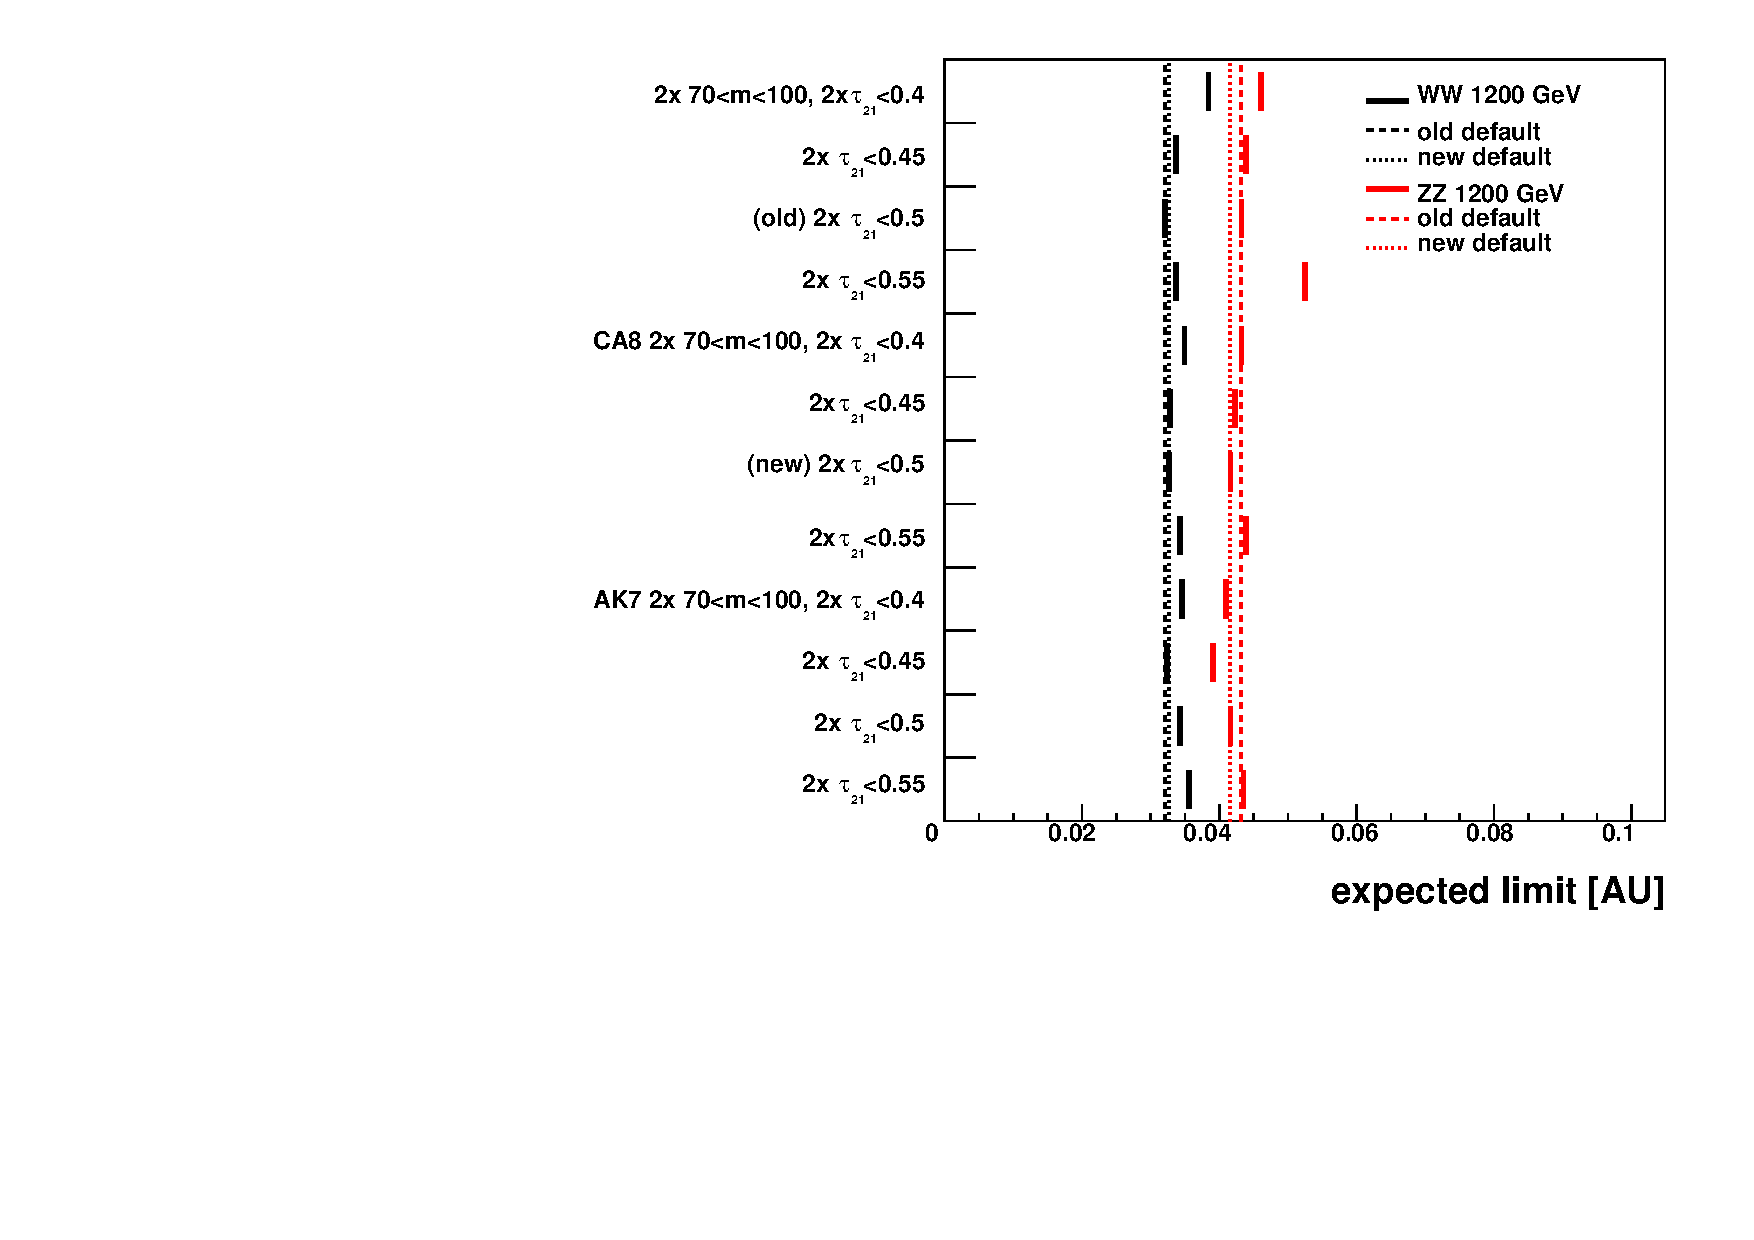
\includegraphics{figs/N-subjettiness/optimization1200_2.pdf}} &
%     \resizebox{0.5\linewidth}{!}{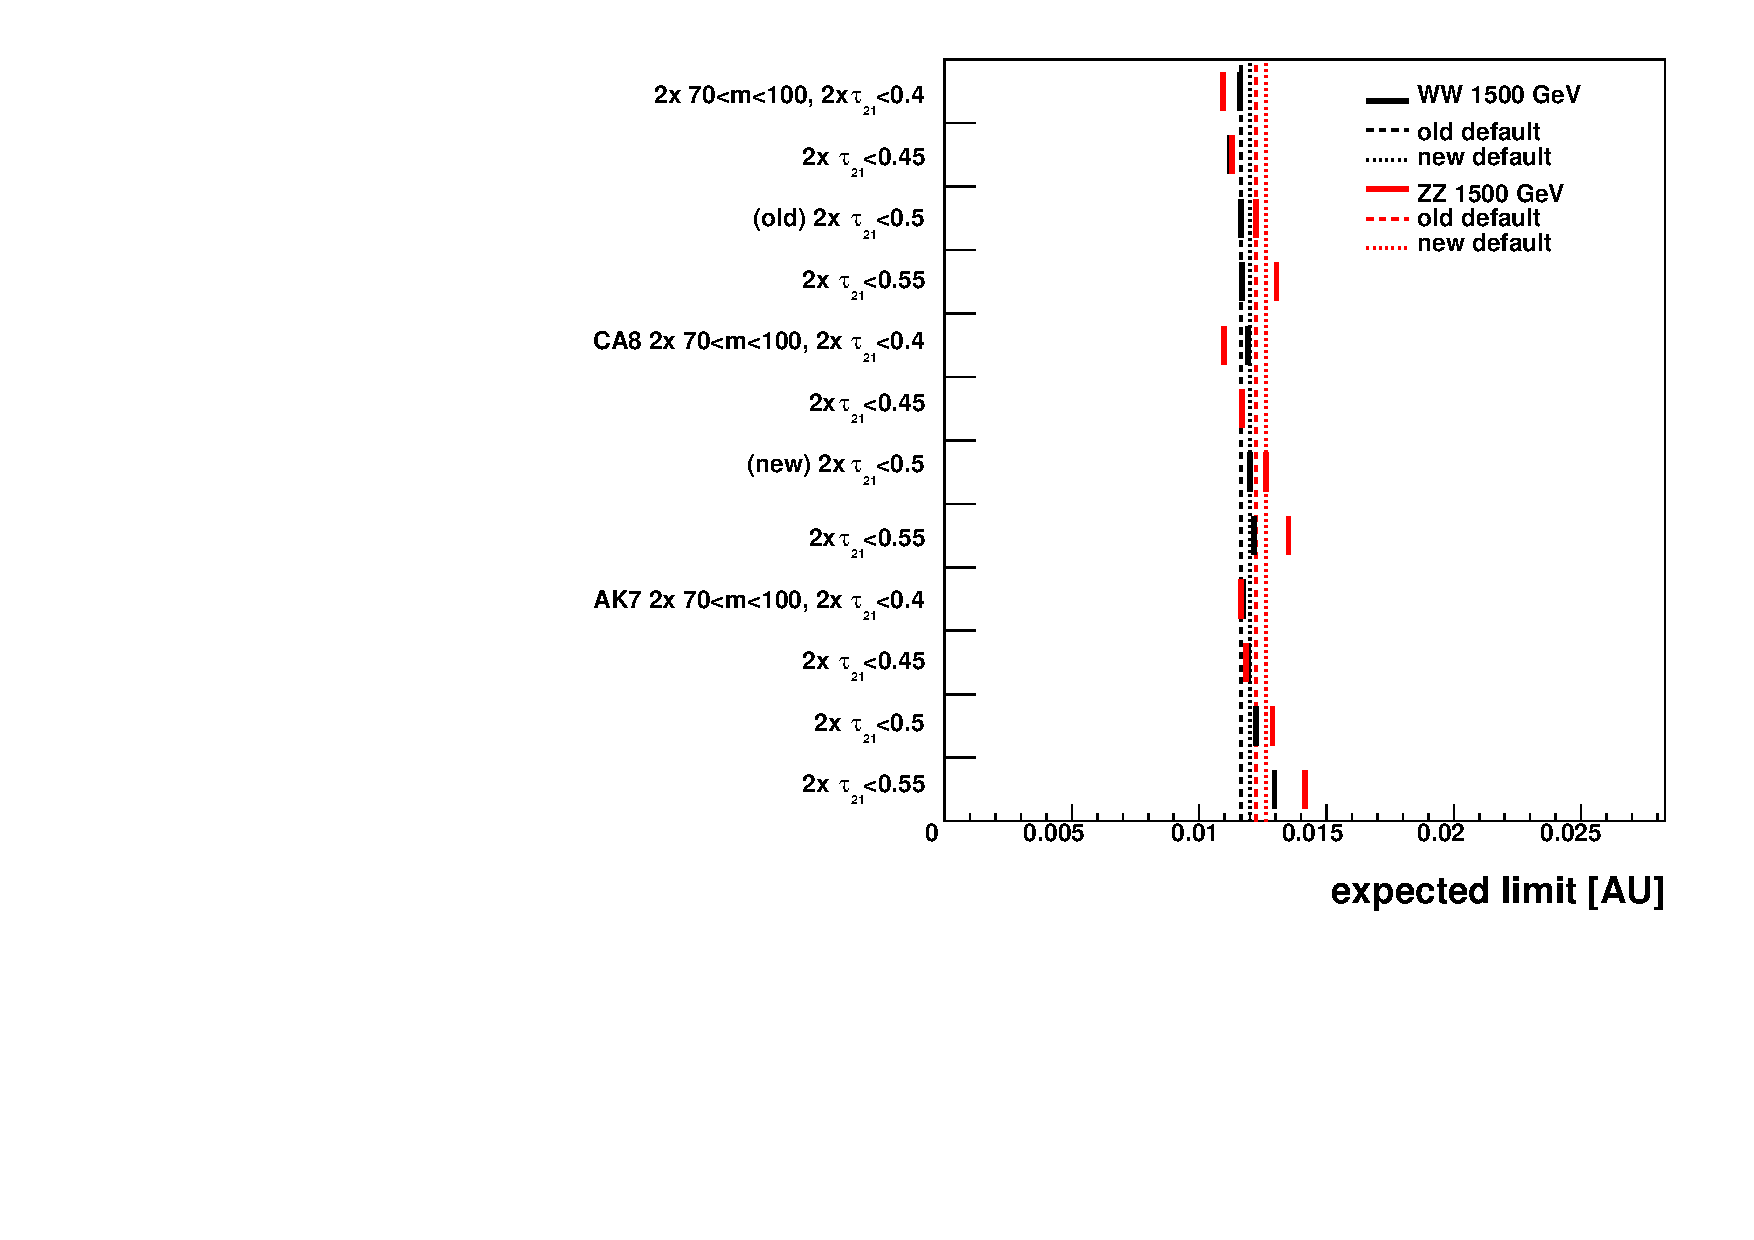
\includegraphics{figs/N-subjettiness/optimization1500_2.pdf}} &
     \resizebox{0.5\linewidth}{!}{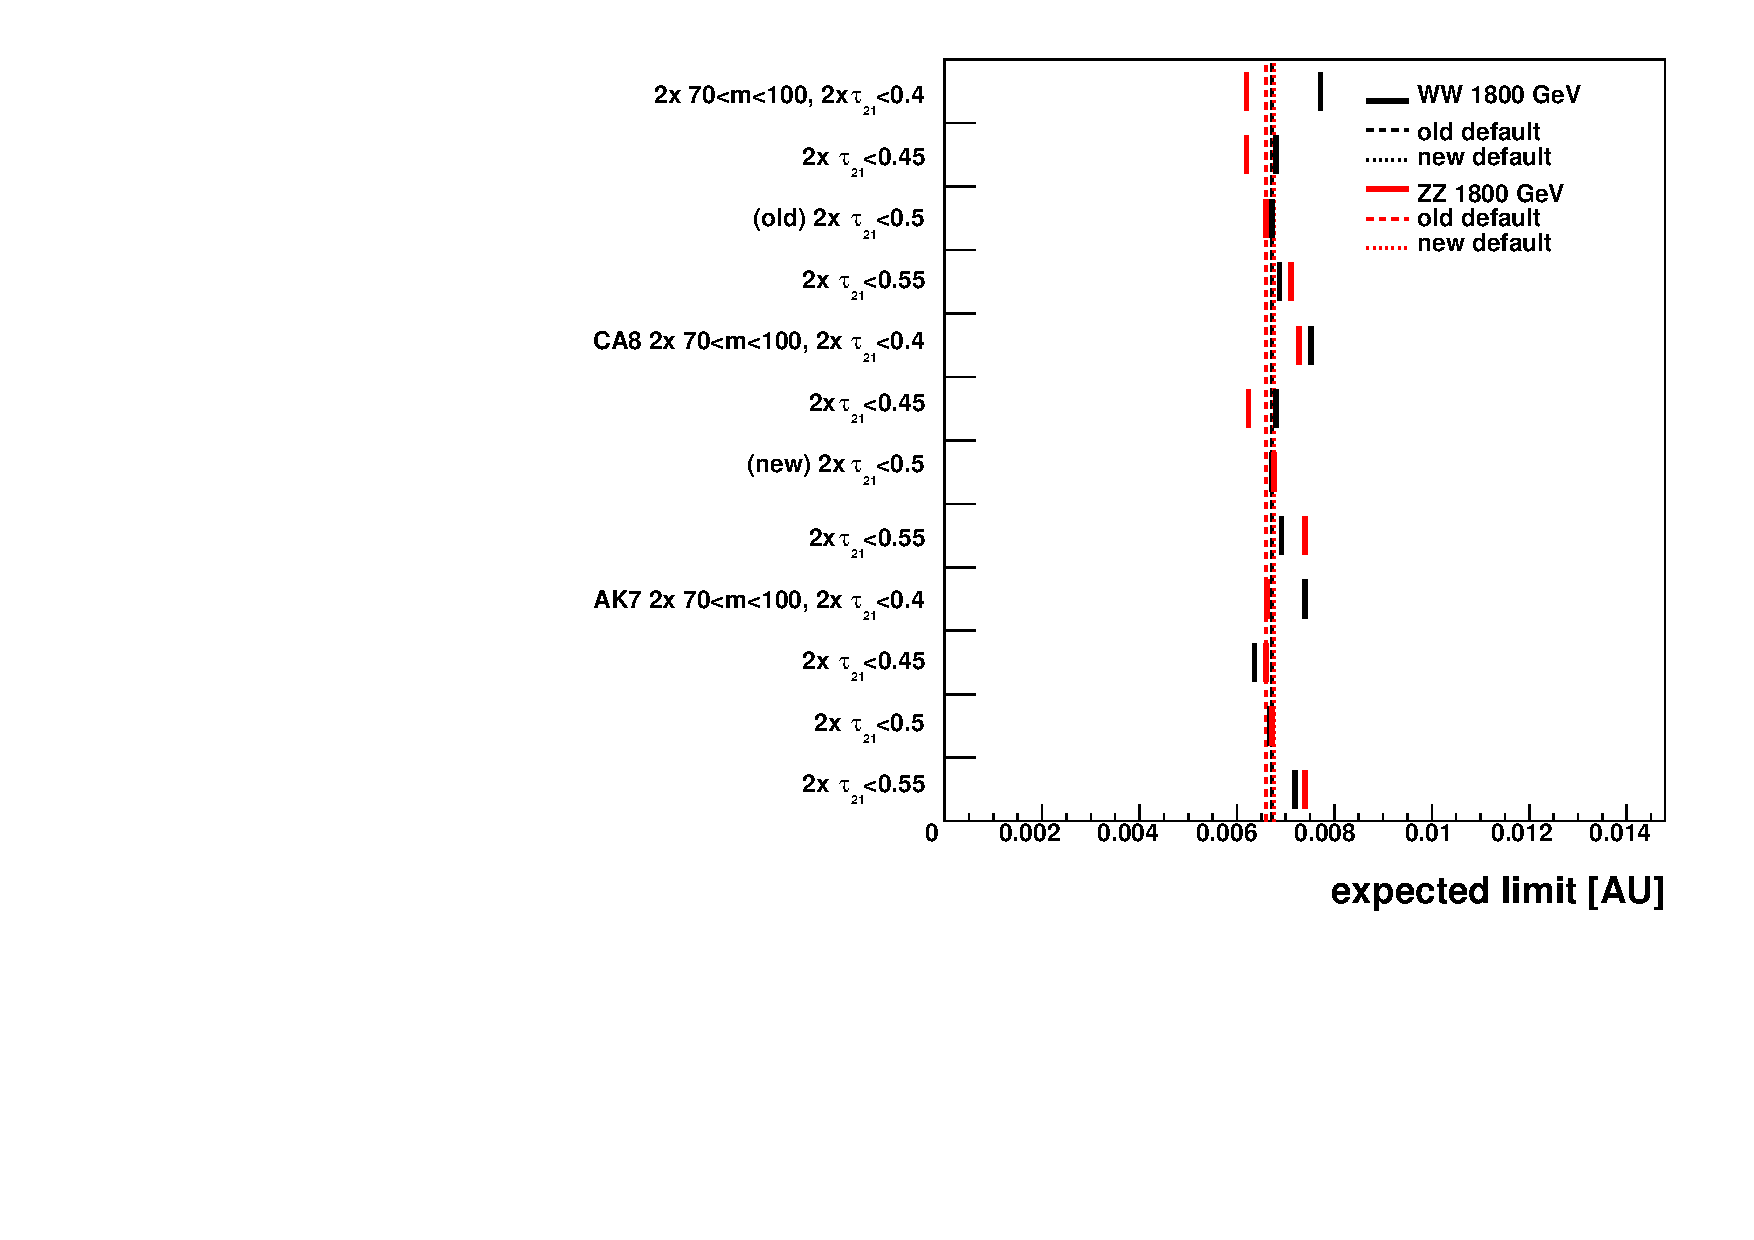
\includegraphics{figs/N-subjettiness/optimization1800_2.pdf}} \\
\end{tabular}
\caption[N-subjettiness]{Comparison of expected limit for different jet algorithms.}
\label{fig:optimization2}
\end{figure}


\label{sec: H tagging}
In the channel of Higgs decays to WW to four quarks, in boosted case, the final four jets will merge to a single fat jet.  And this fat jet will more likely to have four subjets. so our tagger tau4/tau2 is found to be good against top, Z and QCD jets. 
%Figure~\ref{}

 

